\addchap{Introduction}
\label{chapter:introduction}

\addchap{Scientific Computing: a story}
\label{chapter:context}

    %% TODO Historique : https://fr.wikipedia.org/wiki/Superordinateur#Historique_des_records

    \addsec{First computers, from carbon to silicon}%
    \label{sec:first_computers}

        % TODO talk about the human computers, followed by the first (machine) computer created by Cray and IBM, also
        % Von Neuman, analog computers, etc.
        Science has always been tightly associated to computations, hence this is no surprise that the first computers
        were not machines, but humans. Already in the second century AD, Ptolemy, a scientist living in Alexandria,
        wrote the Almagest. This book aggregated the state of the art in mathematics and astronomy and remained a
        reference for centuries. It contained several tables that were computed by the scientist, including a
        trigonometric table (called \emph{table of chords}).

        In 1757, three French astronomers, Clairaut, Lalande and Lepaute, started working on the prediction of the next
        appearances of Halley's comet~\cite[Chapter~1]{human_computers}. Using the recent theories of Newton, they had
        to numerically solve the three-body problem: they computed the orbits of Saturn and Jupiter around the Sun,
        taking into account the attraction force between the two planets. They carried this computation by splitting the
        orbits in tiny steps, computing the new planet locations for each step. They used these sequences of coordinates
        to compute the orbit of Halley's comet around the Sun, by taking into account the effect of the two giant
        planets on the comet and neglecting the effect of the comet itself on the three bodies. They were succesful in
        predicting the next appearance of the comet in the beginning of 1759, making an error of only one month. Their
        work constitutes one of the first recorded division of labor applied to computations, Lalande and Lepaute
        computed the orbits of the two giant planets while Clairaut computed the orbit of the comet.

    \addsec{Exponential growth}%
    \label{sec:exponential_growth}

        % TODO Moore's law, huge performance gains, helped to get great scientifical breakthrough
        % Not terminated yet, we "need" to go further. Side note: when will it be enough? Question of the environmental
        % impact (we make great progress in terms of efficiency, like flops/W, but the growth is even faster (so for
        % instance the total consumptions are still increasing)).

        \begin{figure}[htbp]
            \centering
            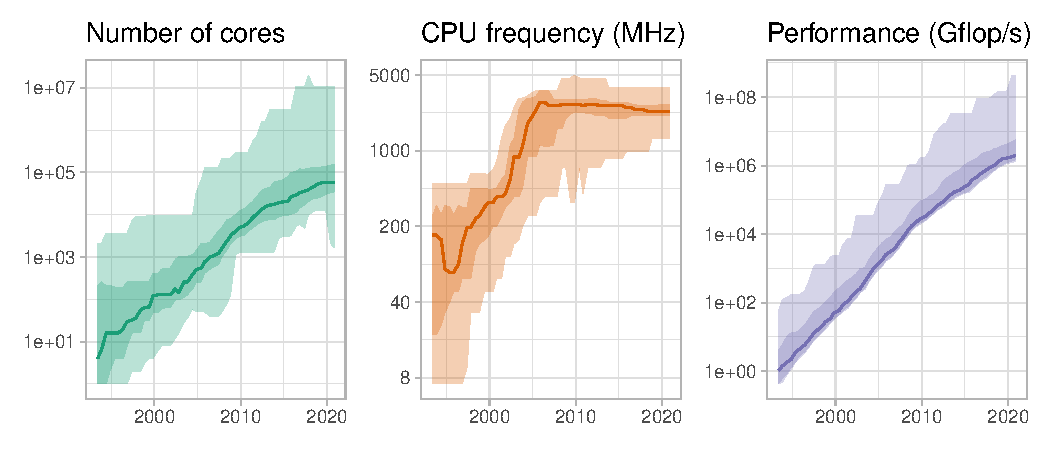
\includegraphics[width=\textwidth]{img/context/top500.pdf}
            \caption{\label{fig:context:top500}
            Both the platform performance and their total number of cores have seen an exponential increase, whereas the CPU
            frequencies have reached a plateau since 15 years}
        \end{figure}


    \addsec{Increased complexity}%
    \label{sec:increased_complexity}

        % TODO increased complexity everywhere (HW and SW), deterministic at micro-level but the macro-level is random
        % no complete understanding of the whole thing, we need experimental CS, we need models (very similarly to what
        % is done in physics or biology)
        Some horror stories\cite{Petrini_2003}\dots
